\chapter{Realizability of Complete Multipartite Graphs}
\label{chap:CompMulti}

The aim of this chapter is to answer the question, "When is a complete multipartite graph realizable?".  A complete answer will not be given, but progress will be made toward an answer.  In particular, a complete multipartite graph is the graph of a polytope if and only if if is either \(K_{1,1}\) or \(K_{2,2}\).  A characterization of all of the possible \(2\)- and \(3\)-faces will also be given.

\section{Hereditary Classes of Graphs}

    A class of graphs \(\mf G\) called a \dfn{hereditary} if \(G\in\mf G\), and \(H\) is an induced subgraph of \(G\) implies \(H\in\mf G\).

    \begin{Example}  Throughout these examples, \(0\notin\N\).
        \begin{enumerate}
            \item   Let \(q\in\N\).  The class of discrete graphs with at most \(q\) vertices is hereditary, and is denoted \(\mf D_q=\setb{D_n}{n\le q}\).
            \item   The class of all discrete graphs is hereditary, and is denoted \(\mf D=\setb{D_n}{n\in\N}\).
            \item   The class of all complete graphs is hereditary, and is denoted \(\mf K=\setb{K_n}{n\in\N}\).
            \item   The class of all complete bipartite graphs (along with the discrete graphs) is hereditary, and is denoted \(\mf K_2=\setb{K_{n,m}}{n,m\in\N}\cup\mf D\).
            \item   Let \(3\le q\in\N\). The class of all complete multipartite graphs with fewer than \(q\) parts (along with the discrete graphs) is hereditary, and is denoted
                    \[
                        \mf K_q=\setb{K_{n_1\dc n_q}}{n_i\in\N\text{ for each }i\in\brac q}\cup\mf K_{q-1}.
                    \]
            \item   Let \(a_1\le a_2\le\dotsb\le a_m\) be a sequence of natural numbers.  Then the class
                \[
                    \mf K[a_1,a_2\dc a_m]=\setb{K_{n_1,n_2\dc n_m}}{n_i\le a_i}\cup\mf K_{m-1}
                \]
                is hereditary.
            \item   Let \(a_1\le a_2\le\dotsb\le a_m\) be a sequence of natural numbers.  Then the class
                \[
                    \mf K(a_1,a_2\dc a_m)=\setb{K_{n_1,n_2\dc n_q}}{q\le m\text{ and }\exists i_1<i_2<\dotsb<i_q\le m\text{ with }n_{i_j}\le a_j}\cup\mf D_{a_m}
                \]
                is hereditary.  More over it is exactly the set of induced subgraphs of the complete multipartite graph \(K_{a_1,a_2\dc a_m}\).
        \end{enumerate}

        \begin{Theorem}\label{Thm:Heredity}
            Suppose \(\mf G\) is a hereditary class of graphs and there is some \(d\in\N\) such that no \(G\in\mf G\) is \(d\)-realizable.  Then for every \(d'>d\) there is no \(G\in\mf G\) which is \(d'\)-realizable.
        \end{Theorem}
        \begin{proof}
            Suppose \(\mf G\) is a hereditary class of graphs and there is some \(d\in\N\) such that no \(G\in\mf G\) is \(d\)-realizable.  Suppose further that there is some \(d'>d\) and a \(G\in\mf G\) such that \(G\) is \(d'\)-realizable.

            Let \(P\) be any \(d'\)-polytope whose graph is \(G\), and let \(F\) be any \(d\)-face of \(P\).  By Theorem \ref{Thm:Induced}, the graph of \(F\) is an induced subgraph of \(G\).  Since \(G\in\mf G\) and \(\mf G\) is hereditary, the graph of \(F\) must also be an element of \(\mf G\).  However this contradicts the assumption that no graph in \(\mf G\) is \(d\)-realizable.
        \end{proof}
    \end{Example}
\section{Complete Bipartite Graphs}

    This section will answer the question "For which values of \(n,m,d\) is the graph \(K_{n,m}\) \(d\)-realizable?".  First, recall the convention that a complete multipartite graph \(K_{n_1,n_2\dc n_t}\) is written such that \(n_1\le n_2\le\dotsb\le n_t\).  Then it will be shown that the answer to the above question is, "only if \(n=m=d\in\seta{1,2}\)".  These are the graphs of \(\simp1\) and \(\xp2\).  Recall that the connectivity of a graph \(\conn G\) is the largest \(q\) such that \(G\) is \(q\)-connected.

    \begin{Lemma}\label{Lem:ConnCompBip}
        \(\conn{K_{n,m}}=n\).
    \end{Lemma}
    \begin{proof}
        Write \(V(K_{n,m})=P\cup Q\) with \(P=\seta{p_1,p_2\dc p_n}\), \(Q=\seta{q_1,q_2\dc q_m}\) and \(E(K_{n,m})=\setb{p_iq_j}{p_i\in P\text{ and }q_j\in Q}\).  Then \(\deg(q_j)=n\) for every \(j\in\brac m\) and \(\deg(p_i)=m\) for every \(i\in\brac n\).  Thus the minimum degree of a vertex of \(K_{n,m}\) is \(n=\min\seta{n,m}\).  Hence \(\conn{K_{n,m}}\le n\).

        To show that \(\conn{K_{n,m}}\ge n\), a set of \(n\) disjoint paths will be constructed for each pair of vertices of \(K_{n,m}\).  There are three cases: a pair of vertices from \(P\); a pair of vertices from \(Q\); and a pair with one vertex in \(P\) and the other in \(Q\).

        In the case that both vertices of the pair are in \(P\), say \(p_i,p_j\), the paths
            \[
                p_i,q_t,p_j\qquad t\in\brac n
            \]
        are disjoint, and there are \(n\) of them.

        In the case that both vertices of the pair are in \(Q\), say \(q_i,q_j\), the paths
            \[
                q_i,p_t,q_j\qquad t\in\brac n
            \]
        are disjoint, and there are \(n\) of them.

        For the case that the pair of vertices is of the form \(p_i,q_j\) with \(p_i\in P\) and \(q_j\in Q\), assume, without loss of generality, that \(i=j=n\).  Then the paths
            \[
                p_n,q_t,p_t,q_n\qquad t\in\brac{n-1}
            \]
        are disjoint, and there are \(n-1\) of them.  These paths, together with the path \(p_n,q_n\) form \(n\) disjoint paths.
    \end{proof}

    \begin{Theorem}\label{Thm:CompBip}
        \(K_{n,m}\) is \(d\)-realizable if and only if \(n=m=d\in\seta{1,2}\).
    \end{Theorem}
    \begin{proof}
        Since \(\card{V(K_{n,m})}\ge 2\), \(K_{n,m}\) is not \((-1)\)-, or \(0\)-realizable.

        Suppose \(n=1\).  Then \(\conn{K_{1,m}}=1\), and thus \(K_{1,m}\) is realizable only if \(d=1\).  There is only one combinatorial type of \(1\)-polytope, and it has graph \(K_{1,1}\).

        Suppose \(n=2\).  Then \(\conn{K_{2,m}}=2\), and thus \(K_{2,m}\) is realizable only if \(d\le2\).  However, \(K_{2,n}\) is never \(1\)-realizable, so if \(K_{2,m}\) is to be \(d\)-realizable, then \(d=2\).  Each \(2\)-polytope has a graph which is a cycle, and thus each vertex has degree \(2\).  The only complete bipartite graph for which each vertex has degree \(2\) is \(K_{2,2}\), and it is the graph of \(\xp2\), the \(2\)-crosspolytope.

        Suppose \(n\ge3\).  Then \(K_{n,m}\) is  at least \(3\)-connected.  Suppose that \(K_{n,m}\) is \(3\)-realizable.  Steinitz's Theorem (Theorem \ref{Thm:Steinitz}) thus implies that \(K_{n,m}\) must be planar.  However this is not possible since \(K_{n,m}\) has an induced \(K_{3,3}\) for \(n\ge3\) (and therefore a \(K_{3,3}\) minor).  Thus \(K_{n,m}\) is never \(3\)-realizable.

        Ergo, by Theorem \ref{Thm:Heredity}, \(K_{n,m}\) is not \(d\)-realizable for \(d\ge3\).
    \end{proof}

\section{Complete \protect$3\protect$-partite Graphs}
    The proof of the following lemma is similar to that of lemma \ref{Lem:ConnCompBip}.
    \begin{Lemma}
        \(\conn{K_{1,n,m}}=n+1\)
    \end{Lemma}

    \begin{Theorem}\label{Thm:KOneNM}
        \(K_{1,n,m}\) is \(d\)-realizable if and only if \(K_{n,m}\) is \((d-1)\)-realizable.
    \end{Theorem}
    \begin{proof}
        Suppose that \(n=1\).  Then \(\conn{K_{1,1,m}}=2\), and \(K_{1,1,m}\) is only a cycle if \(m=1\).  In which case it is the graph of \(\simp2\), the \(2\)-simplex.

        Suppose that \(n=2\).  The graph \(K_{1,2,2}\) is the graph of \(\pyr{\xp2}\).  If \(m\ge 3\), then \(K_{1,2,m}\) cannot be the graph of a \(3\)-polytope since it would then be a \(3\)-polytope with \(3+m\) vertices and an \(m\)-anticlique (see Theorem \ref{Thm:Anticliques}).  The graph \(K_{1,2,m}\) also cannot be \(d\)-realizable for \(d>3\) since \(\conn{K_{1,2,m}}=3\).

        Suppose that \(n=3\).  The graph \(K_{1,3,m}\) then has an induced \(K_{3,3}\), and therefore cannot be planar (hence is not \(3\)-realizable).  Furthermore, \(K_{1,3,m}\) cannot be the graph of a \(4\)-polytope since it has \(1+3+m=4+m\) vertices and an \(m\)-anticlique.

        Suppose that \(n\ge4\), and write
            \[
                V(K_{1,n,m})
                    =
                        \seta{a}                \cup
                        \setb{b_i}{i\in\brac n} \cup
                        \setb{c_i}{i\in\brac m}.
            \]
        where each set in the union above is one of the sets of vertices in the definition of a complete bipartite graph.  Here again, \(K_{1,n,m}\) has an induced \(K_{3,3}\), and is therefore not \(3\)-realizable.  Suppose that \(K_{1,n,m}\) is the graph of a \(4\)-polytope \(P\).  Then the set of induced subgraphs of \(K_{1,n,m}\) is \(\mf K(1,n,m)\) which is hereditary.  The only graph in \(\mf K(1,n,m)\) that is \(3\)-realizable is \(K_{1,2,2}\), and therefore each facet of \(P\) must be a pyramid over a quadrilateral.  In order to obtain an induced \(K_{1,2,2}\) from \(K_{1,n,m}\), the set of vertices must be of the form \(\seta{a,b_{i_1},b_{i_2},c_{j_1},c_{j_2}}\).  However this forces the vertex \(a\) to be in each facet, and this is impossible.

        Thus no graph of the form \(K_{1,n,m}\) is \(4\)-realizable, and therefore no graph \(K_{1,n,m}\) is \(d\)-realizable for \(d\ge 4\).
    \end{proof}

    The graphs \(K_{2,2,m}\) are not \(4\)-realizable since they would then have \(2+2+m=4+m\) vertices and an \(m\)-anticlique.  More generally, \(K_{2,n,m}\) is not \((2+n)\)-realizable.

    The \(K_{2,n,m}\) case is more difficult.  First, note that a graph of this form is only planar if \(n=m=2\), and in this case is the graph of \(\xp3\), the \(3\)-crosspolytope.

    Suppose that \(K_{2,n,m}\) is the graph of some polytope \(P\).  Working with the hereditary class of graphs \(\mf K(2,n,m)\) (this is the set of induced subgraphs of \(K_{2,n,m}\)) shows that the \(2\)-faces of \(P\) must be either \(2\)-simplices, or \(2\)-crosspolytopes.  Similarly, the \(3\)-faces of \(P\) can only be pyramids over quadrilaterals, or \(3\)-crosspolytopes.  Further, \(P\) has at most one facet that is combinatorially equivalent to \(\xp3\) since each \(\xp3\) facet must contain both vertices in the color class of cardinality \(2\).  This restriction of the allowable facets does not show that there is no such polytope.  A proof of the following theorem can be found in \cite{PerShep}.
        \begin{Theorem}[Perles, Shephard]
            If \(P\) is a \(d\)-polytope with \(d+2\) or fewer vertices, then there is a \((d+1)\)-polytope all of whose facets are combinatorially equivalent to \(P\).
        \end{Theorem}
    The authors also prove, in the same paper, that for \(d\ge6\) there is no \((d+1)\)-polytope all of whose facets are combinatorially equivalent to \(\xp d\).

    Suppose \(P\) is a \(4\)-polytope with graph \(K_{2,3,3}\) and that \(P\) has a facet combinatorially equivalent to \(\xp3\).  Then by a careful consideration of the possible ridges, it can be shown that there must be a ridge that is contained in only one facet.  Therefore there is no \(4\)-polytope with graph \(K_{2,3,3}\), and hence no polytope with graph \(K_{2,3,3}\).  Alternatively, the two papers \cite{Alts:Quasi} and \cite{Alts:Complete} provide a complete list of all \(4\)-polytopes with \(8\) vertices.  These papers show that any such polytope is either quasisimplicial (all of its facets are simplicial), or has a facet that is a simplex.  Since a realization of \(K_{2,3,3}\) could satisfy neither of these properties, there can be no such polytope.

    \subsection{Complete \protect$k\protect$-partite Graphs \protect$(k>3)\protect$}
    In general, if \(P\) is a realization of a complete multipartite graph, then every one of its \(2\)-faces must be combinatorially equivalent to either \(\simp2\) or \(\xp2\) since these are the only complete multipartite graphs that are cycles.  Similarly, every one of its \(3\)-faces must be combinatorially equivalent to one of the following:
        \begin{itemize}
            \item   a \(3\)-simplex, or
            \item   a pyramid over \(\xp2\), or
            \item   a bipyramid over a \(2\)-simplex, or
            \item   a \(3\)-crosspolytope
        \end{itemize}
    since these are the only planar, \(3\)-connected complete multipartite graphs.

    A direct consequence of Theorem \ref{Thm:Anticliques} is that if \(K_{n_1,n_2\dc n_t}\) is \(d\)-realizable, then \(d<\sum_{i\in\brac{t-1}}n_i\).  If \(K_{n_1,n_2\dc n_t}\) is \(d\)-realizable as a polytope \(P\), then \(K_{1,n_1,n_2\dc n_t}\) is \(d+1\)-realizable as a pyramid over \(P\).  The converse is, unfortunately, not true since \(K_{1,1,1,2}\) is the graph of \(\cyc53\) (i.{}e.{}, a bipyramid over a \(2\)-simplex) but \(K_{1,1,2}\) is not the graph of any polytope.  Similarly, \(K_{n_1,n_2\dc n_t,2}\) is realizable as a bipyramid over \(P\).

    Thus, if (as a set) \(\seta{n_1,n_2\dc n_t}\sbset\seta{1,2}\), then \(K_{n_1,n_2\dc n_t}\) is the graph of a polytope if and only if (as a multiset) \(\seta{n_1,n_2\dc n_t}\) is not equal to either \(\seta{1,2}\) or \(\seta{1,1,2}\).

    \begin{Conjecture}
        If \(K_{n_1,n_2\dc n_t}\) is the graph of a polytope, then \(\seta{n_1,n_2\dc n_t}\sbset\seta{1,2}\) as sets,.
    \end{Conjecture}

    Note that the conjecture does not make mention of the dimension of the polytope.  This is because the graphs of higher-dimensional crosspolytopes can be realized in multiple dimensions.

\section{Graphs of Crosspolytopes}
    Throughout this section, let \(G_n\) denote the graph of the \(n\)-dimensional crosspolytope for \(n\ge 2\), that is
        \[
            G_n
                =   \gr{X_n}
                =   K_{\underbrace{2,2\dc2}_n}.
        \]
    The goal of this section will be to establish for which \(d\) the graph \(G_n\) is \(d\)-realizable.

    The graphs \(G_2\) and \(G_3\) are realizable only in dimensions \(2\) and \(3\) respectively.  Thus assume throughout that \(n\ge 4\).  The first thing to do is establish an upper bound on the values \(d\) such that \(G_n\) is \(d\)-realizable.  Recall the Hadwiger number of a graph \(G\) is \(\had G=\max\setb{n}{K_n\text{ is a minor of }G}\).  Theorem \ref{Thm:CompleteMinor} then implies:
    \begin{Cor}\label{Cor:HadBound}
        If a graph \(G\) is \(d\)-realizable, then \(d\le\had G-1\).
    \end{Cor}

    Thus a natural question to ask is "What is \(\had{G_n}\)?".  This question was answered in \cite{Halin}.

    \begin{Theorem}[Halin 1966]\label{Thm:Halin}
        \[\had{G_n}=\floor{\frac{3n}2}.\]
    \end{Theorem}
        The following gives, for each \(n\), an explicit construction of a maximal complete minor of \(G_n\).

        Write \(V(G_n)=V_1\cup V_2\) where \(V_1=\seta{v^1_1,v^1_2\dc v^1_n}\) and \(V_2=\seta{v^2_1,v^2_2\dc v^2_n}\) are disjoint sets such that
            \begin{align*}
                E(G_n)
                    &=  \setb{v^i_jv^k_l}{i,k\in\brac2,\,j,l\in\brac n\text{, and if }i\ne k\text{, then }j\ne l}\\
                    &=  \binom{V(G_n)}2\setminus\setb{v^1_jv^2_j}{j\in\brac n}.
            \end{align*}
        Set
            \begin{align*}
                D
                    &=  \setb{v^i_jv^2_k}{i\in\brac2,\,j,k>\floor{n/2}}
                            \cup    \setb{v^i_jv^2_k}{i\in\brac2,\,j\le\floor{n/2}\text{ and }k>\floor{n/2}\text{ with }j+k\ne n+1}
            \end{align*}
        and
            \begin{align*}
                C
                    &=  \setb{v^2_iv^2_j}{i+j=n+1}.
            \end{align*}
        Then \((G_n\setminus D)/C\) is a complete graph with \(\floor{3n/2}\) vertices.  The paths
            \begin{align*}
                &   v^1_iv^1_j              &   &   i,j\in\brac n\\
                &   v^2_iv^2_j              &   &   i,j\le\floor{n/2}\\
                &   v^1_iv^2_j              &   &   i\in\brac n, j\le\floor{n/2}\text{ with }i\ne j\\
                &   v^1_iv^2_{n+1-i}v^2_i   &   &   i\le\floor{n/2}
            \end{align*}
        contract to form the edges in the complete graph.  Thus \(h(G_n)\ge\floor{3n/2}\).  This construction is included here because \cite{Halin} does not give an explicit construction of a maximal complete minor.  See Figures \ref{Fig:Xfour} and \ref{Fig:Xfive} for examples of these constructions.
        \begin{figure}[h!bt]
            \centering
                \includegraphics[width=.5\textwidth, page=30]{pictures.pdf}
            \caption{\protect$G_4\protect$, edges in the deletion set are dotted, and those in the contraction set are dashed.\label{Fig:Xfour}}
        \end{figure}

        \begin{figure}[h!bt]
            \centering
                \includegraphics[width=.7\textwidth, page=31]{pictures.pdf}
            \caption{\protect$G_5\protect$, edges in the deletion set are dotted, and those in the contraction set are dashed.\label{Fig:Xfive}}
        \end{figure}
        \subsection{High Dimensional Realizations}

            The graph \(G_n\) \emph{could} thus be realizable in each dimension from \(4\) to \(\floor{3n/2}-1\).  Before giving explicit constructions of \(d\)-polytopes with graph \(G_n\) for \(n\le d<\floor{3n/2}\), notice that if \(p_i\in\N\) with \(p_i\ge 2\) and \(\sum_{i\in\brac m}p_i=q\), then
                \[
                    \gr{\xp{p_1}\join\xp{p_2}\join\dotsb\join\xp{p_m}}=G_q
                \]
            and
                \[
                    \dim(\xp{p_1}\join\xp{p_2}\join\dotsb\join\xp{p_m})=\sum_{i\in\brac m}p_i+m-1.
                \]
            In particular, let \(\xp2^k\) be the join of \(k\) copies of \(\xp2\), so that \(\gr{\xp2^k}=G_{2k}\) and \(\dim\xp2^k=3k-1\).  Thus the polytope \(\xp{3n-2d}\join\xp2^{d-n}\) is a \(d\)-polytope with graph \(G_n\).  These polytopes are by no means unique with these properties.  Others can be constructed by similar means by taking joins of crosspolytopes (or even polytopes with these graphs) and forcing the joins to have the required number of vertices and be of the required dimension.  That is:
                \begin{Theorem}
                    The graph \(G_n\) is \(d\)-realizable for \(n\le d<\ds\floor{\frac{3n}2}\).
                \end{Theorem}
            
            This settles the question of \(d\)-realizability of \(G_n\) for \(d\ge n\).  However, the number of combinatorial types of \(d\)-polytopes with graph \(G_n\) and \(d\ge n\) is not known.  These constructions merely provide a lower bound for that number.


            The following is a Corollary to Theorems \ref{Thm:Anticliques} and \ref{Thm:Halin}.
                \begin{Cor}
                    Let \(P\) be a simple \(d\)-polytope that is not a simplex. If \(\gr P=K_{n_1,n_2\dc n_s}\), then \(P=X_2\).
                \end{Cor}
                \begin{proof}
                    If \(P\) is simple, then \(\deg\ve v=d\) for every \(\ve v\in\vrt P\).  Therefore \(\sum_{j\in\brac s\setminus\seta i}n_j=d\) for every \(i\in\brac s\).  Hence \(n_1=n_2=\dotsb=n_s=k\).  Since \(P\) is not a simplex, \(k\ne1\).  Notice that \(P\) is  a \(d\)-polytope with \(d+k\) vertices whose graph has a \(k\)-anticlique.  Thus \(k=2\).  Now, \(P\) is a \(2(s-1)\)-polytope with graph \(G_s\).  Therefore
                        \[
                            2(s-1)\le\floor{\frac{3s}2}-1\le\frac{3s}2-1.
                        \]
                    Solving for \(s\) yields \(s\le2\).  Hence \(s=2\), whence \(\gr P=G_2\).  Thence \(P=X_2\).
                \end{proof}

        \subsection{Low Dimensional Realizations}

            In \cite{GrunBook}, a construction of a \(4\)-polytope \(Z\) with graph \(G_5\) is given.  Repeated bipyramids over this polytope yield \((n-1)\)-realizations of \(G_n\) for \(n\ge 5\).  Note that \(Z\join \xp2\) is a \(7\)-polytope with graph \(G_7\) and is not \(\xp7\).  Thus, in general, the graph \(G_n\) is not the graph of a unique \(n\)-polytope.  The polytope \(Z\) has an additional property that will be useful in talking about low dimensional realizations of \(G_n\).

            \begin{Definition}
                A polytope \(P\) is called \dfn{centrally symmetric} if there is a point \(\ve p\in P\) such that \(\ve x\in P-\ve p\) implies \(-\ve x\in P-\ve p\).
            \end{Definition}

            It will be assumed throughout that \(\ve p=\ve 0\).  The \(4\)-realization \(Z\) of \(G_5\) is centrally symmetric and much of the work on low-dimensional realizations of \(G_n\) concerns centrally symmetric realizations.   In \cite{GrunBook} it is shown that if \(G_6\) is \(4\)-realizable by a polytope \(P\), then \(P\) cannot be centrally symmetric.

            Let \(P\) be a centrally symmetric \(d\)-polytope with graph \(G_n\) with \(n<d\).  The polytope \(P\join\xp2\) is a \((d+3)\)-polytope with graph \(G_{n+2}\).  However, \(P\join\xp2\) is not centrally symmetric.

            It is shown in \cite{BarNov:CSCyclic} that if \(P\) is a  centrally symmetric \(d\)-polytope with \(N\) vertices, then
                \[
                    f_1(P)
                        \le
                            \frac{N^2}2(1-2^{-d}).
                \]
            In the case that \(\gr P=G_n\), this implies that \(\binlog n\le d\) where \(\binlog n\) is the binary logarithm \(\log_2 n\).

            Let \(m\in\N\).  The paper \cite{BarLeeNov:Many} gives an explicit construction of a \(d\)-dimensional centrally symmetric polytope with graph \(G_n\) where
                \begin{align*}
                    d
                        &=
                            4m+6\\
                    n
                        &=
                            2\cdot3^{m+1}.
                \end{align*}
            This construction, in the case \(m=0\), yields that the polytope \(\xp6\) has graph \(G_6\).  Setting \(m=1\) gives a centrally symmetric \(10\)-polytope with graph \(G_{18}\).  By considering bipyramids over these polytopes, one obtains centrally symmetric polytopes of dimension \(4m+7\) with graph \(G_n\) where \(n=2\cdot3^{m+1}+1\).  Furthermore, taking a join  with \(\xp2\) yields a polytope of dimension \(4m+11\) and with graph \(G_n\) where \(n=2\cdot3^{m+1}+2\). 